\documentclass[conference]{IEEEtran}
\IEEEoverridecommandlockouts
% The preceding line is only needed to identify funding in the first footnote. If that is unneeded, please comment it out.
\usepackage{cite}
\usepackage{amsmath,amssymb,amsfonts}
\usepackage{algorithmic}
\usepackage{graphicx}
\usepackage{textcomp}
\usepackage{xcolor}
\def\BibTeX{{\rm B\kern-.05em{\sc i\kern-.025em b}\kern-.08em
    T\kern-.1667em\lower.7ex\hbox{E}\kern-.125emX}}
\begin{document}

\title{ Low-Supply Voltage Sensor with an Optical Indicator: Design, Construction, and Analysis}

\author{\IEEEauthorblockN{1\textsuperscript{st} Miguel Villa Floran}
\IEEEauthorblockA{\textit{Computer Engineering Department} \\
\textit{California Polytechnic State University, San Luis Obispo}\\
San Luis Obispo, United States of America \\
miguel.villafloran@gmail.com}
}

\maketitle

\begin{abstract}
This experiment focuses on the design, construction, and analysis of a low-supply voltage sensor-indicator circuit employing a Zener diode based voltage limiter and LED indicator. Key components include a 4.3 V Zener diode, TLC3702 voltage comparator IC, and a multi-turn potentiometer. The circuit utilizes a linear voltage divider and Zener diode to monitor supply voltage, activating an LED when the voltage drops below a specified threshold. The experiment providing valuable insights into the functionality and performance of the designed circuit


\end{abstract}

\begin{IEEEkeywords}
Zener diode, voltage comparator, LED, linear voltage divider, voltage limiter
\end{IEEEkeywords}

\section{Introduction}

\subsection{Voltage Comparator}

The voltage comparator is a device that specializes in comparing the voltages of two incoming signals and producing a high or low output voltage to indicate which is larger. If the the voltage across the positive terminal $V_{in+}$ is greater than the voltage across the negative terminal $V_{in-}$, the voltage comparator generate a logical high output voltage $V_{DD}$. Otherwise, a logical low output voltage $V_{SS}$ is produced \cite{week6}.

The voltage comparator is utilized in this design to indicate whether the voltage supply drops below a specified threshold, which for our intents and purposes is 8 V.

\subsection{Voltage Limiting Zener Diode}
The Zener Diode exhibits similar behaviors and properties as the standard PN junction diode. However, Zener diodes are also designed to have a well-defined and sharp reverse breakdown voltage, also referred to as the Zener voltage ($V_z$). When a Zener diode connected across a circuit in reverse bias reaches its Zener voltage, it maintains its Zener voltage and behaves as a closed circuit regardless of current fluctuations and changes in voltage. It is safe to use a Zener Diode in breakdown so long as the power it dissipates is below its maximum power rating \cite{week7}.

\begin{figure}[htbp]
\centerline{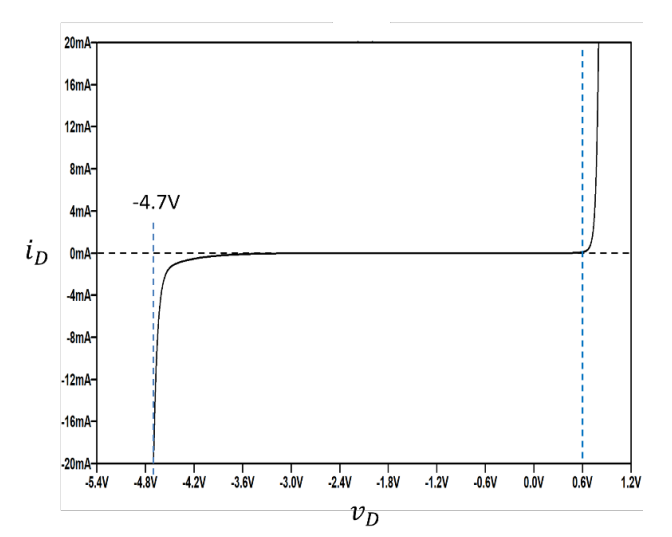
\includegraphics{./images/vi-characteristics.png}}
\caption{VI Characteristic of the 4.3V Zener Diode. \cite{week7}}
\label{fig}
\end{figure}

The reverse breakdown properties of a Zener Diode are leveraged to create voltage limiters for regulating the voltage across sensitive components or provide constant reference voltages \cite{week7}. This is done by connecting a resistor, which limits the current coming into the diode, in series to the Zener Diode, which is connected in parallel to the load. In this design, the Zener Diode provides a constant voltage across the negative terminal of the comparator \eqref{eq_1}.

\begin{equation}
V_- \approx V_Z\label{eq_1}
\end{equation}


\subsection{Multi-Turn Potentiometer}

A multi-turn rotary potentiometer is a type of voltage divider whose resistance changes as it is rotated, allowing for variable control of the output voltage in electronic circuits. The 

This adjustable resistance is utilized in this circuit so that the positive terminal's voltage is equivalent to the negative terminal's voltage, which is equivalent to the Zener voltage so that the comparator is tripped at the threshold voltage. The values of the potentiometer can also be found mathematically by using \eqref{eq_3}, but was found experimentally.

\begin{equation}
V_+ = \frac{R_a}{R_a + R_b} V_{DD}\label{eq_2}
\end{equation}

\begin{equation}
V_{DD(trip)} = (1 + \frac{R_b}{R_a})V_{Z}\label{eq_3}
\end{equation}

\subsection{LED Optical Indicator}

The light-emitting diode (LED) indicator serves as a visual cue, activating when the supply voltage falls below the predetermined threshold. The LED is reverse-biased relative to the output of the comparator and its cathode is connected to the supply voltage to ensure it only lights up when the supply voltage drops below the threshold voltage. When the supply voltage is above the threshold voltage, the comparator outputs the supply voltage, and the LED does not activate as there is no potential difference across it. When the supply voltage is below the threshold voltage, the comparator outputs 0 V, and the LED activates as there is a potential difference across it. To ensure the LED does not burn out, a resistor is added to limit current coming into the LED. This resistance is found by using \eqref{eq_4}, where 

\begin{equation}
R_{LED} \approx \frac{V_{DD(trip)} - V_{LED}}{I_{LED}}\label{eq_4}
\end{equation}

\section{Sensor Test and Data}

This experiment required a single circuit to be assembled and tested in four phases as shown in figures \ref{circuit1}, \ref{circuit2},  \ref{circuit3}, and \ref{circuit4} to ensure its proper functionality and performance. For all circuits, the comparator was implemented using a TLC3702 voltage comparator IC, the optical indicator was implemented using a WP7113ID 617nm Red LED, the voltage limiter was implemented using a 1N5229BTR 4.3 V Zener Diode, and the voltage divider was implemented using a 5.00E-250 multi-turn potentiometer.

The first phase involved the assembly of the Zener-based voltage limiter, as depicted in figure \ref{circuit1}. The bias direction of the diode was validated and the limiter was verified to produce a constant output equivalent to its Zener voltage.

\begin{figure}[htbp]
\centerline{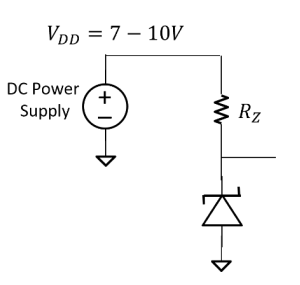
\includegraphics{./images/circuit1.png}}
\caption{Schematic with the Zener-based limiter assembled and validated during phase 1. \cite{week7}}
\label{circuit1}
\end{figure}

The second phase involved the assembly of the linear voltage divider, as depicted in figure \ref{circuit2}. The potentiometer's knob was adjusted until the voltage difference between the positive and negative terminal is close to zero when the supply voltage is equivalent to the threshold voltage.

\begin{figure}[htbp]
\centerline{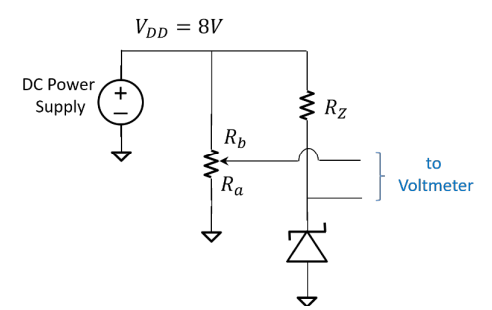
\includegraphics{./images/circuit2.png}}
\caption{Schematic with the linear voltage divider assembled and validated during phase 2. \cite{week7}}
\label{circuit2}
\end{figure}

The third phase involved the assembly of the voltage comparator, as depicted in figure \ref{circuit3}. The comparator was verified to switches states at the threshold voltage.

\begin{figure}[htbp]
\centerline{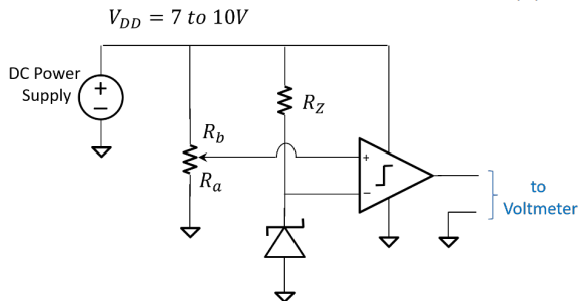
\includegraphics{./images/circuit3.png}}
\caption{Schematic with the linear voltage divider assembled and validated during phase 3. \cite{week7}}
\label{circuit3}
\end{figure}

The fourth phase involved the assembly of the voltage comparator, as depicted in figure \ref{circuit3}. The comparator was verified to switches states at the threshold voltage.

\begin{figure}[htbp]
\centerline{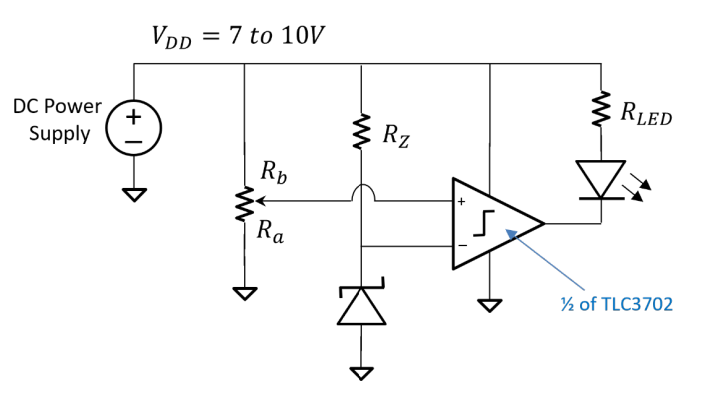
\includegraphics{./images/circuit4.png}}
\caption{Schematic with the linear voltage divider assembled and validated during phase 4. \cite{week7}}
\label{circuit4}
\end{figure}


\subsection{Figures and Tables}
\paragraph{Positioning Figures and Tables} Place figures and tables at the top and 
bottom of columns. Avoid placing them in the middle of columns. Large 
figures and tables may span across both columns. Figure captions should be 
below the figures; table heads should appear above the tables. Insert 
figures and tables after they are cited in the text. Use the abbreviation 
``Fig.~\ref{fig}'', even at the beginning of a sentence.

\begin{table}[htbp]
\caption{Table Type Styles}
\begin{center}
\begin{tabular}{|c|c|c|c|}
\hline
\textbf{Table}&\multicolumn{3}{|c|}{\textbf{Table Column Head}} \\
\cline{2-4} 
\textbf{Head} & \textbf{\textit{Table column subhead}}& \textbf{\textit{Subhead}}& \textbf{\textit{Subhead}} \\
\hline
copy& More table copy$^{\mathrm{a}}$& &  \\
\hline
\multicolumn{4}{l}{$^{\mathrm{a}}$Sample of a Table footnote.}
\end{tabular}
\label{tab1}
\end{center}
\end{table}

\begin{figure}[htbp]
\centerline{\includegraphics{images/fig1.png}}
\caption{Example of a figure caption.}
\label{fig}
\end{figure}

Figure Labels: Use 8 point Times New Roman for Figure labels. Use words 
rather than symbols or abbreviations when writing Figure axis labels to 
avoid confusing the reader. As an example, write the quantity 
``Magnetization'', or ``Magnetization, M'', not just ``M''. If including 
units in the label, present them within parentheses. Do not label axes only 
with units. In the example, write ``Magnetization (A/m)'' or ``Magnetization 
\{A[m(1)]\}'', not just ``A/m''. Do not label axes with a ratio of 
quantities and units. For example, write ``Temperature (K)'', not 
``Temperature/K''.

\begin{thebibliography}{00}
\bibitem{week6} Week 6: Elementary Logic Circuits - Part II, Available https://canvas.calpoly.edu/courses/113173/files?preview=11616452
\bibitem{week7} Week 7: A Low-Supply Voltage Sensor with an Optical Indicator, Available https://canvas.calpoly.edu/courses/113173/files?preview=11699080
\end{thebibliography}
\vspace{12pt}

\end{document}
